\documentclass[12pt]{article}
\usepackage[margin=1in]{geometry}
\usepackage{array}
\usepackage{float}
\usepackage{caption}
\usepackage{enumitem}
\usepackage{subcaption}
\usepackage[table, dvipsnames]{xcolor} 
\usepackage{graphicx}
\usepackage{longtable}
\usepackage{ltxtable}
\usepackage{wasysym}
\usepackage{tabularx}
\usepackage{cleveref}
\title{Project 50 Music Playlist Manager}
\date{}
\begin{document}
	\maketitle
	\noindent
	\textbf{Team with Github names:}
	\begin{itemize}[leftmargin=0.0cm,labelsep=0.2cm]
		\item[] Badam-Osor Khaltar (badamosor)
		\item[] Paul McCumber (paulmccumber)
		\item[] Luke Meszar (lukemeszar)
	\end{itemize}
	\textbf{Vision:} Provide a platform for building and sharing music playlists.
	\section{Project Description}
	Sharing playlists of music between a large group of people can be difficult when
	everyone doesn't listen to music through the same service. This will allow people to create
	playlists in a generic format that can then be integrated into the user’s service of choice. This allows people to share their playlists with their friends who can then export it into the streaming service of their choice. 
	\section{Completed Requirements}
	\rowcolors{2}{blue!10}{white}
	\begin{table}[H]
		\centering
		\label{tab:urc}
		\caption*{User Requirements}
		\begin{tabularx}{450pt}{lXl}
			ID & Description & Priority\\\hline
			UR-01 & Users can create account & High \\
			UR-02 & Users can create a playlist & High \\
			UR-03 & Users can search database for song title, album title,
			artist, and playlist name & High \\
			UR-04 & Users can add content (songs, from albums or artists) to a playlist (only songs can be added) & High \\
			UR-06 & Users can make playlists collaborative & Low \\
			UR-07 & Users can share a playlist & High \\
			UR-11 & Users can export playlists into Spotify (through a fake API backend) & High \\
			UR-12 & Users can export playlists into Tidal (through a fake API backend) & High \\
			UR-13 & Users can export playlists into Google Play Music (through a fake API backend) & High \\
		\end{tabularx}
	\end{table}
	\begin{table}[H]
		\centering
		\label{tab:nfrc}
		\caption*{Non-Functional Requirements}
		\begin{tabularx}{450pt}{lXl}
			ID & Description & Priority\\\hline
			NFR-01 & Search has to be less than 20ms & High \\
			NFR-03 & Should be able to expand to other music services easily & Medium \\
		\end{tabularx}
	\end{table}
	\LTXtable{450pt}{functionalTableCompleted}
	\section{Incomplete Requirements}
	\rowcolors{2}{blue!10}{white}
	\begin{table}[H]
		\centering
		\label{tab:uri}
		\caption*{User Requirements}
		\begin{tabularx}{450pt}{lXl}
			ID & Description & Priority\\\hline
			UR-05 & Users can remove songs from a playlist & Medium \\
			UR-08 & Users can register their Spotify account to our service & High \\
			UR-09 & Users can register their Tidal account to our service & High \\
			UR-10 & Users can register their Google Play Music account to our service & High \\
		\end{tabularx}
	\end{table}
	\begin{table}[H]
		\centering
		\label{tab:nfri}
		\caption*{Non-Functional Requirements}
		\begin{tabularx}{450pt}{lXl}
			ID & Description & Priority\\\hline
			NFR-02 & Service should support thousands of concurrent users & High \\
		\end{tabularx}
	\end{table}
	\LTXtable{450pt}{functionalTableIncomplete}
	\section{Class Diagrams}
	\begin{figure}[H]
		\centering
		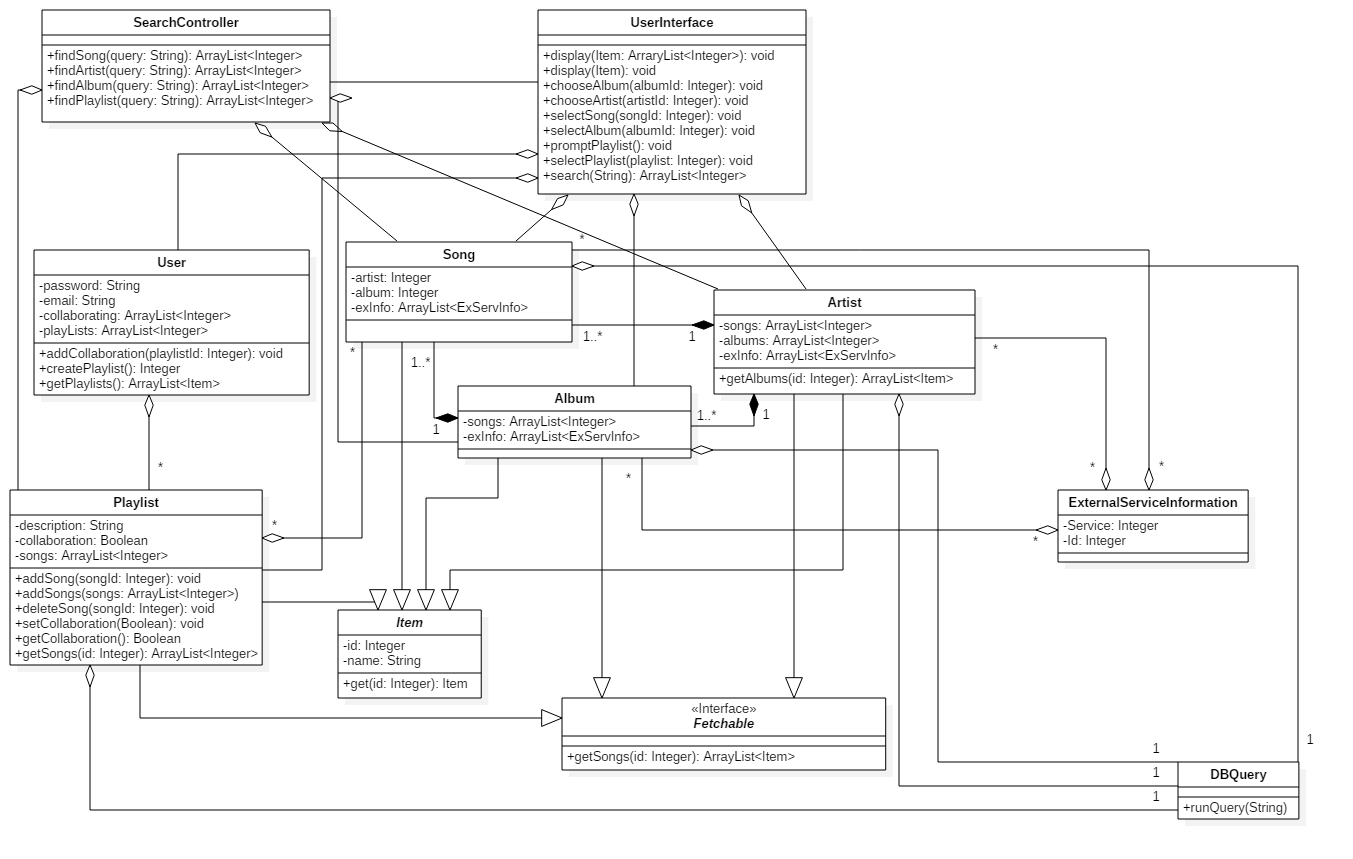
\includegraphics[scale=0.35]{MusicManagerClassDiagram.png}
		\caption{Class Diagram from Part 2}
		\label{fig:classDiagPart2}
	\end{figure}
	Our class diagram changed significantly between Part 2 and now. The fundamental reason for this is we started working with the Django framework after we finished the Part 2. Since Django had a lot of built of functionality for accessing data from a database and then displaying that data, we incorporated our ideas from Part 2 into this framework. We also updated the class diagram to reflect the design patterns we had implemented. 
	
	The class diagram in \Cref{fig:classDiagCompleted} is entirely completed. The green classes are classes that are implemented by Django so there are no details included. The blue classes represent a larger set of classes that didn't fit in this diagram. They can be seen in detail in \Cref{fig:classDiagExport} and \Cref{fig:classDiagSearch} respectively. 
	\begin{figure}[H]
		\centering
		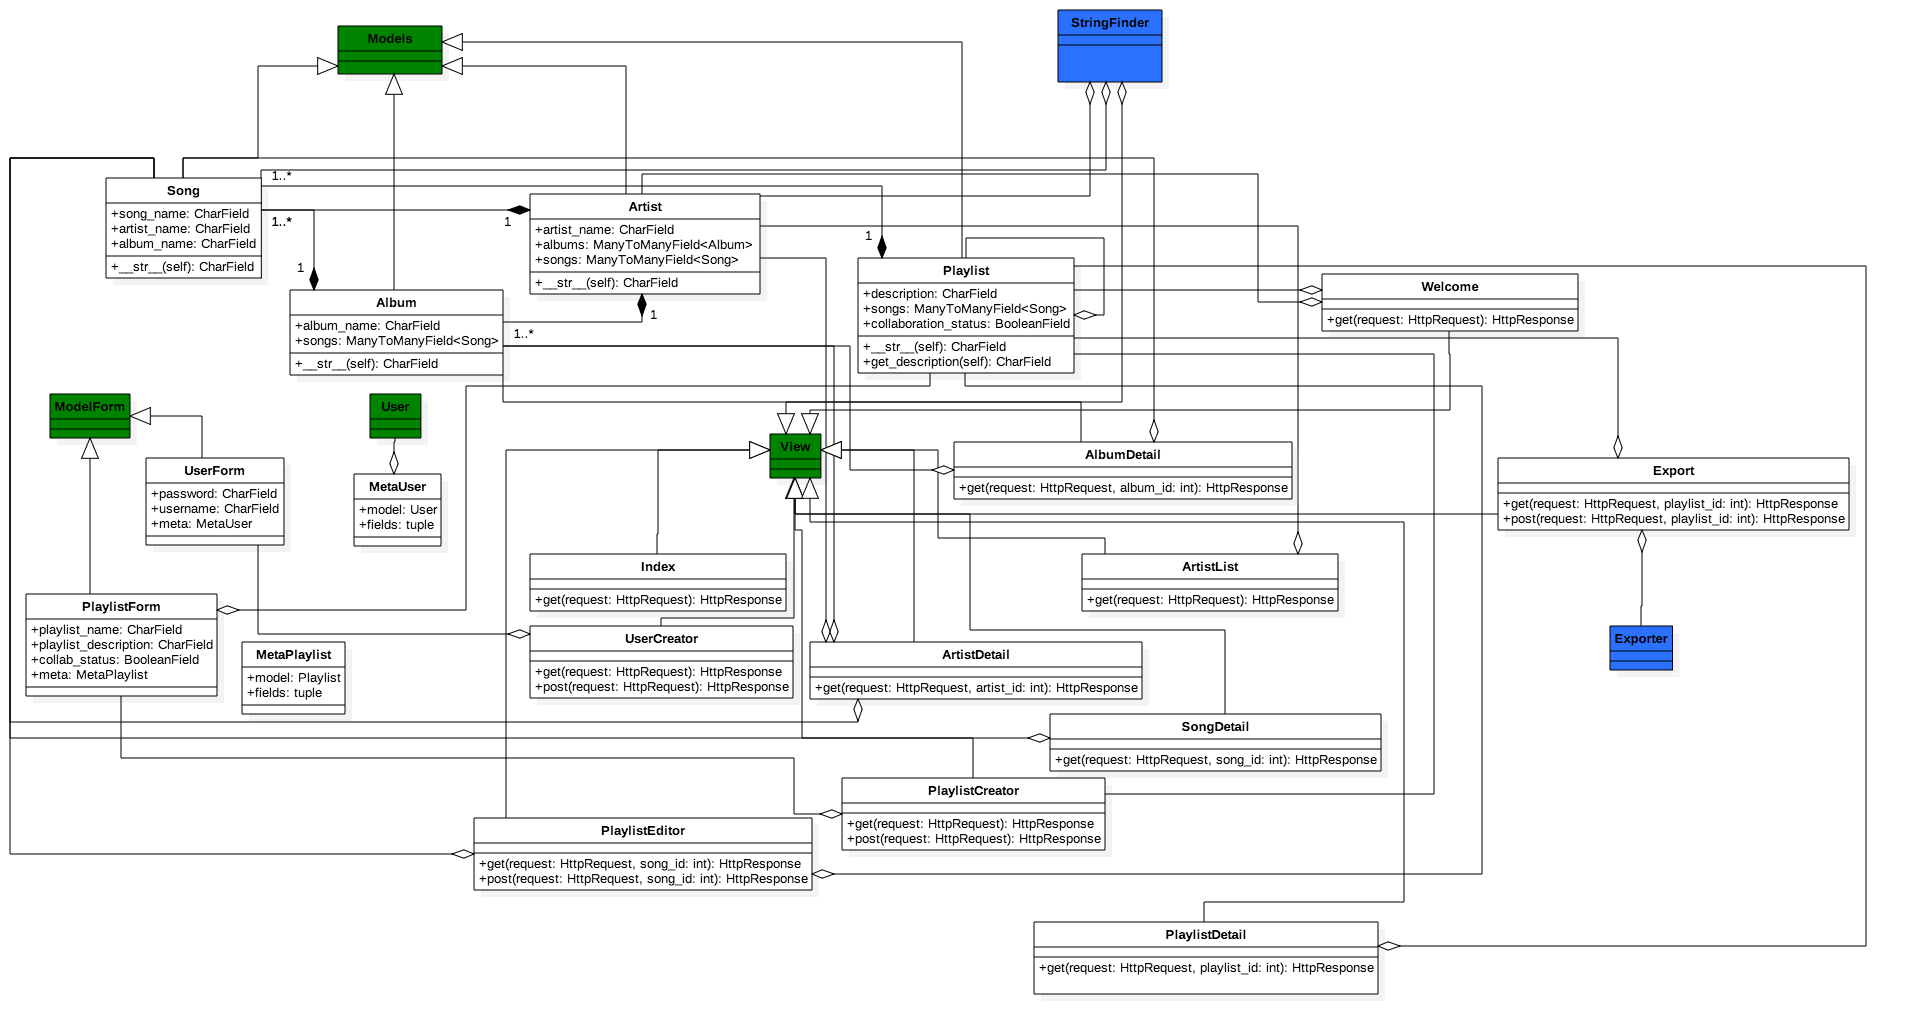
\includegraphics[scale=0.25]{DiagramAddedSearch.png}
		\caption{Class Diagram Completed}
		\label{fig:classDiagCompleted}
	\end{figure}
	\begin{figure}[H]
		\centering
		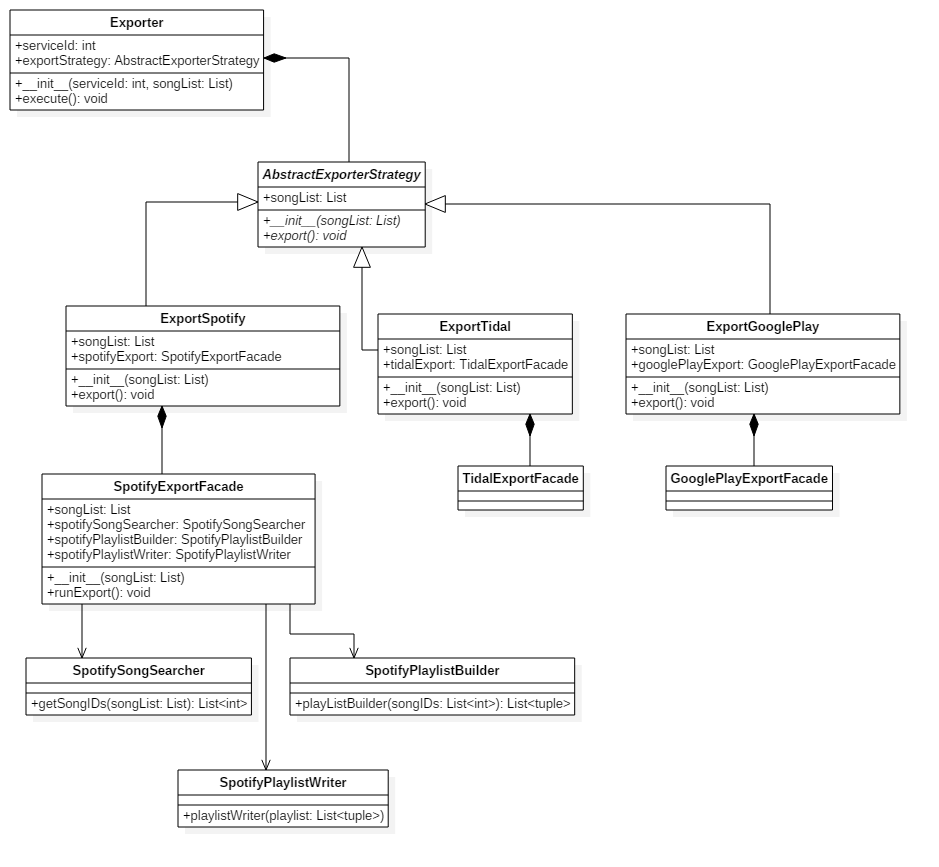
\includegraphics[scale=0.25]{ExportClassDiagram.png}
		\caption{Class Diagram for Export}
		\label{fig:classDiagExport}
	\end{figure}
	\begin{figure}[H]
		\centering
		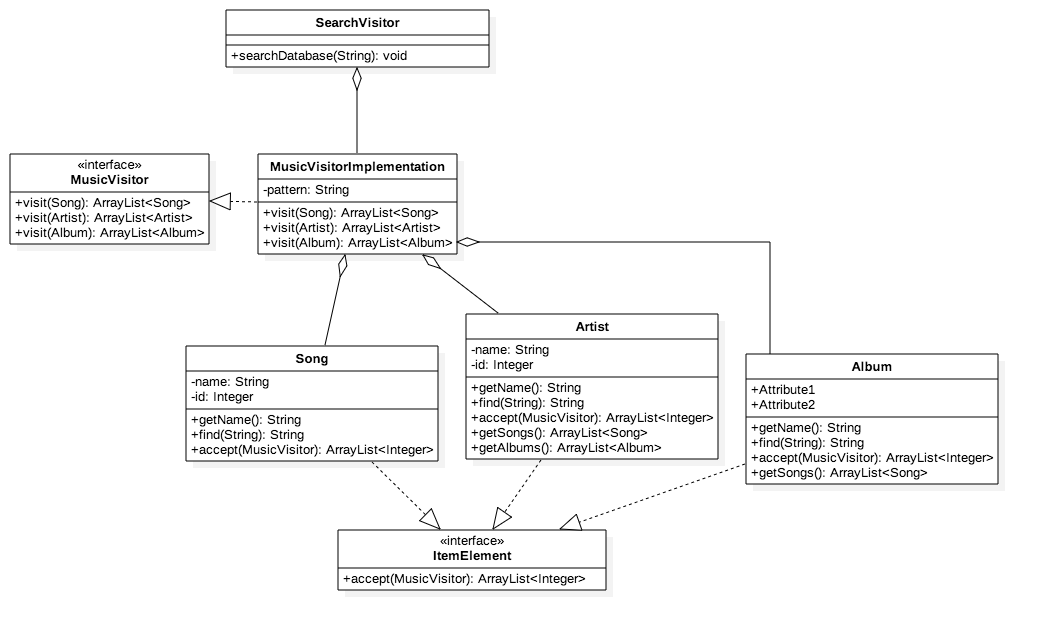
\includegraphics[scale=0.25]{Search.png}
		\caption{Class Diagram for Search}
		\label{fig:classDiagSearch}
	\end{figure}
	\section{Design Patterns}
	\begin{figure}[H]
		\centering
		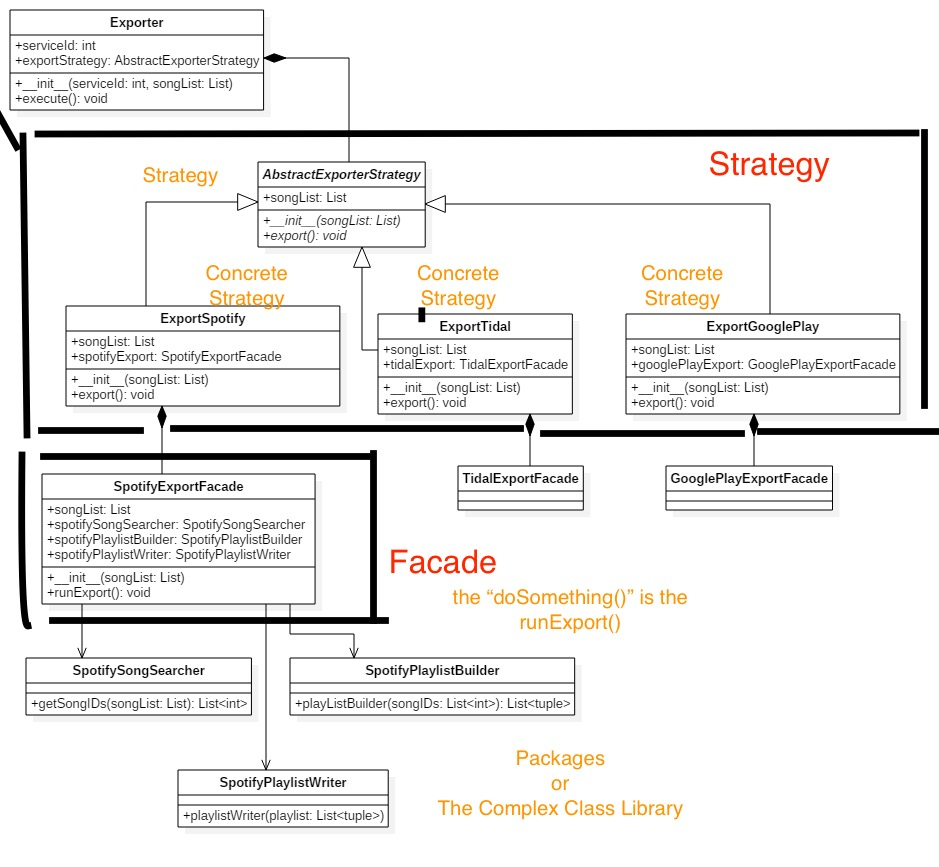
\includegraphics[scale=0.25]{ExportClassDiagram.jpg}
		\caption{Class Diagram for Export with Strategy and Facade Patterns Highlighted}
		\label{fig:classDiagExportPattern}
	\end{figure}
	We used the Strategy pattern as a way to choose which external service we wanted to export to and use the appropriate algorithm for it. This was combined with the Facade pattern to handle the complexities of exporting a playlist. This allowed us to make a nice interface that didn't care about all the nitty-gritty details of exporting. This pattern would be even more important if we had worked with the actual music service API's where things would have been even more complicated. 
	\begin{figure}[H]
		\centering
		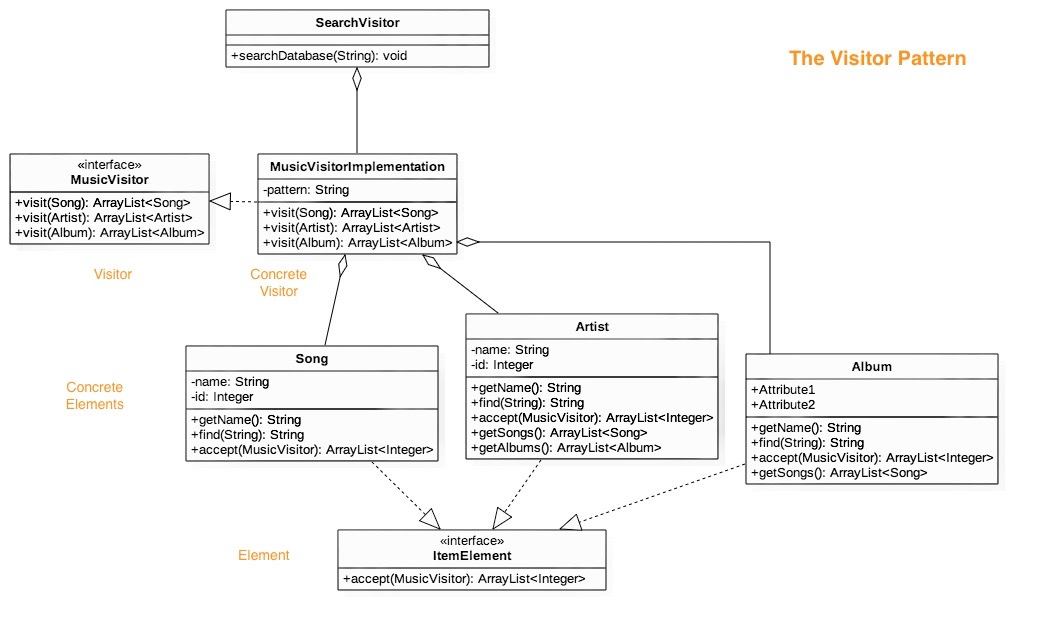
\includegraphics[scale=0.25]{Search.jpg}
		\caption{Class Diagram for Search with Visitor Pattern Highlighted}
		\label{fig:classDiagSearchPattern}
	\end{figure}
	We decided to implement Visitor pattern for search.  We created a visitor class that implements all the specialization of searching or Artist, Song, and Album data without having to modify the classes themselves (other than implementing the ItemElement interface with the accept()).  The MusicVisitorImplementation instead did the searching and built the lists of matches that could be rendered to the search results page in a fashion that can be used in content editing.    
	\section{What We Learned}
	
	Our choice to use the Django framework had a significant impact on our original design.  Much of the work we did in Part 2 and even Part 3 ended up being thrown out.  This  comes from learning aspects of the MVC after we did Part 2.  The framework make managing the data much different than we originally designed.  We ended up having to not only change our class diagrams but much of the prototyping we had done was thrown out as well.  
	
	Even so, the work we did in Part 2 and Part 3 made the work in proceeding with Django much easier.  Plus we had some tools for working with the database and ideas about the flow that had been worked out and prototyped that made implementation much easier.  When converting the classes for Artist, Song, Album, and Playlist into Django Models (essentially Python representations for database objects), not a lot of thinking had to be done since we had already done it in Part 2.  
	
	Plus, everyone on the team enjoyed the opportunity of getting some exposure to an MVC.
	Throughout this project, we learned the importance of planning ahead.
	
	Overall, having the design on paper before hand made planning and communicating as a team easier. It was easier to decide who was going to implement what when we had concrete ideas of what needed to be implemented based on the analysis. One of the most useful parts was the requirements analysis. Having a list of things we wanted to get done from the beginning made for a lot simpler plan going forward. It was very nice to be able to check items off a list as we completed them. Overall, doing the analysis and design made the who process a lot smoother than it would have been if you had just jumped straight in. 
\end{document}